\documentclass[nohyperref]{article}
\usepackage[utf8]{inputenc}
\usepackage[T1]{fontenc}
\usepackage{xcolor}
\usepackage{amsmath, amsthm, amssymb}
\usepackage{tikz}
\usetikzlibrary{patterns}
\usetikzlibrary{automata, positioning}
\usetikzlibrary{shapes,decorations,arrows,calc,arrows.meta,fit,positioning}
\tikzset{
    -Latex,auto,node distance =1 cm and 1 cm,semithick,
    state/.style ={circle, draw, minimum width = 0.8 cm},
    state2/.style ={circle, draw, minimum width = 0.1 cm, inner sep=0pt},
    point/.style = {circle, draw, inner sep=0.04cm,fill,node contents={}},
    bidirected/.style={Latex-Latex,dashed},
    el/.style = {inner sep=2pt, align=left, sloped}
}

\begin{document}

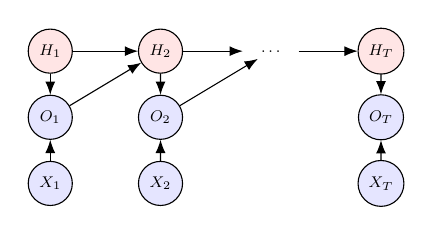
\begin{tikzpicture}[scale=.7,transform shape]
    \node[state,fill=red!10!white] (h1) at (0,0) {\footnotesize $H_1$};
    \node[state,fill=red!10!white] (h2) at (2,0) {\footnotesize $H_2$};
    \node[draw=none, minimum width = 1 cm] (hdots) at (4,0) {\footnotesize $\ldots$};
    \node[state,fill=red!10!white] (hT) at (6,0) {\footnotesize $H_T$};
    \node[state,fill=blue!10!white] (o1) at (0,-1.2) {\footnotesize $O_1$};
    \node[state,fill=blue!10!white] (o2) at (2,-1.2) {\footnotesize $O_2$};
    \node[state,fill=blue!10!white] (oT) at (6,-1.2) {\footnotesize $O_T$};
    \node[state,fill=blue!10!white] (x1) at (0,-2.4) {\footnotesize $X_1$};
    \node[state,fill=blue!10!white] (x2) at (2,-2.4) {\footnotesize $X_2$};
    \node[state,fill=blue!10!white] (xT) at (6,-2.4) {\footnotesize $X_T$};
    \path (h1) edge (o1);
    \path (h1) edge (h2);
    \path (o1) edge (h2);
    \path (h2) edge (o2);
    \path (h2) edge (hdots);
    \path (o2) edge (hdots);
    \path (hT) edge (oT);
    \path (hdots) edge (hT);
    \path (x1) edge (o1);
    \path (x2) edge (o2);
    \path (xT) edge (oT);
\end{tikzpicture}

\end{document}